\documentclass[11pt]{article}

% First load extension packages
\usepackage[a4paper,margin=25mm]{geometry}    % page layout
\usepackage{setspace}
%\onehalfspacing % line spacing
\singlespacing
\usepackage{amsfonts,amssymb,amsmath} % useful math extensions
\usepackage{graphicx} % graphics import
\usepackage{siunitx} % easy SI units
\usepackage{subcaption}
\usepackage[noabbrev]{cleveref}

\usepackage{rotating}

% Change paragraph indentation
\setlength{\parskip}{10pt}
\setlength{\parindent}{0pt}

% Bibliography
\usepackage[style=ieee,backend=biber,citestyle=numeric-comp,sorting=nty,doi=false,url=false,isbn=false]{biblatex}
\addbibresource{references.bib}
\usepackage[utf8]{inputenc}
\usepackage[T1]{fontenc}

% User-defined commands
\newcommand{\diff}[2]{\frac{\mathrm{d}{#1}}{\mathrm{d}{#2}}}
\newcommand{\ddiff}[2]{\frac{\mathrm{d}^2{#1}}{\mathrm{d}{#2}^2}}
\newcommand{\pdiff}[2]{\frac{\partial{#1}}{\partial{#2}}}
\newcommand{\pddiff}[2]{\frac{\partial^2{#1}}{\partial{#2}^2}}
\newcommand{\pdiffdiff}[3]{\frac{\partial^2{#1}}{\partial{#2}\partial{#3}}}
\renewcommand{\vec}[1]{\boldsymbol{#1}}
\newcommand{\Idx}{\;\mathrm{d}x}
\newcommand{\Real}{\mathbb{R}}
\newcommand{\Complex}{\mathbb{C}}
\newcommand{\Rational}{\mathbb{Q}}
\newcommand{\Integer}{\mathbb{Z}}
\newcommand{\Natural}{\mathbb{N}}

% topmatter

\title{Modelling the Instabilities of Pilot-Operated\\Pressure Relief Valves  \vspace{-20pt}}

\author{James Roff \\ Supervised by Prof. Alan Champneys \vspace{-10pt}}

\date{\today}


% main body
\begin{document}
\maketitle
\vspace{-50pt}

\section{Introduction}

Pressure Relief Valves (PRVs) are an important safety feature in many pressurised systems, forming a final defence against over pressurisation. A fluid operating at a higher pressure than designed can lead to decreases in efficiency for some processes. More severely, a fluid within a vessel reaching high pressures can cause an explosive release of fluid. This has two serious impacts. Firstly, severe damage can cause costly repairs possibly including replacing the entire pressure tank. There is not only the capital cost of repairs, but also the potential loss of revenue for being unable to use a process. Secondly, it could prove fatal to an unfortunate operator.

The simplest type of PRV is the direct spring-operated PRV. These are widely used, and rely on a spring to hold a poppet in place. As the pressure increases, a greater force acts upon the poppet to open the valve. Hence, the poppet will rise which allows fluid to escape causing the pressure in the tank to be relieved. PRVs are widely used as they prevent unnecessary waste of fluid because the valve will close once the pressure has decreased. However, spring-operated PRVs do not scale well for larger vessels as larger flow rates are needed requiring a very large physical space.

A more complex design of PRV is the Pilot-Operated PRV (see \cref{fig: Diagram} below). This allows fluid both above and below the piston, and so uses the fluid pressure to keep the valve shut. When the pressure becomes too great, a small pilot valve opens which reduces the pressure above the piston. Hence, the main valve opens allowing the fluid to escape and relieve the pressure in the vessel. This has several advantages. Even for large tanks, no physical spring is needed, so the valve can be physically smaller than a spring-operated PRV.

Unfortunately, both spring and pilot operated PRVs do not always behave as expected. Several forms of instability exist, ranging from a desirable blow-down effect to the most damaging chatter instability~\cite{Hos2017DynamicRecommendations}. A blow-down effect is when the PRV closes at a lower pressure than that at which it opens, called the set pressure. This is desirable as it can help the valve remain slightly open rather than cycling, where the valve intermittently opens and closes.

The more damaging chatter instability is characterised by high frequency oscillations in which the poppet or piston undergoes impacts. These oscillations contain large amounts of energy, which can cause severe damage to the PRV. This damage can decrease the performance of the valve, or even cause it to fail completely. These consequences have serious repercussions for the pressurised vessel as the final safety precaution is compromised, meaning the dangerous effects of over pressurisation may occur.

This project aims to study the various types of instability which can occur for a pilot-operated PRV. Particular focus is placed on identifying the damaging chatter instability. If successful in establishing a stability criteria, this work will allow a PRV to be designed to avoid chatter. This report will begin by reviewing the current understanding surrounding instability in PRVs.

%what are you working on?
%what is the real-world challenge?
%why should anyone care?
% \section{Literature review}

% % don't need to look at since
% % instabilities are well known
% % research is conclusive
% 
A review of the current literature on both direct spring-operated and pilot-operated PRVs is now presented. The existence of unstable operation for pressure relief valves (PRVs) has been a known phenomena since the 1960s (for example, see \cite{Kasai1968OnSystem}).
%, with early analysis believing a resonance occurred between the valve and operating fluid~\cite{KASAI1968OnSystem}.
As the simplest type of  PRV, a large amount of analysis has been performed on direct spring-operated PRVs \cite{Kasai1968OnSystem,Thomann1976OscillationsPipe,Hayashi1995InstabilityCircuit,Darby2013TheModel,Bazso2013AnValve,Erdodi2017PredictionModelling,Hos2015ModelPipe,Hos2017DynamicRecommendations}. A combination of mathematical analysis and experimental results have been used to study these instabilities. Computational simulations have helped  in two ways; first by allowing full fluid dynamical equations
%which cannot be solved analytically
to be investigated (for example \cite{Erdodi2017PredictionModelling,Hos2015ModelPipe}). Second, when combined with reduced order models analysis such as numerical continuation to identify bifurcations can be performed (for example \cite{Hos2015DynamicModelling}).

%\subsection{Direct spring-operated PRVs}
\section{Direct spring-operated PRVs}

One of the earliest works by Kasai~\cite{Kasai1968OnSystem} used the Fourier domain to analysis a spring-operated PRV, performing some experimental validation of the analysis. Later work using similar techniques identified that acoustic waves were induced by the valve~\cite{Thomann1976OscillationsPipe}. These early works incorrectly believed that chatter occurred due to a resonance between the valve and the operating fluid.

Later work by Hayashi~\cite{Hayashi1995InstabilityCircuit} demonstrates the potential of numerical simulations. The paper demonstrated that numerical simulations could reproduce the valve dynamics, including chatter. Furthermore, numerical continuation produced a bifurcation diagram, identifying a period-doubling route to chaotic behaviour. That behaviour was further analysed using experimental studies~\cite{Bazso2013AnValve}. More recent numerical solutions consist of complex Computation Fluid Dynamic (CFD) models, with Erd\H{o}di and H\H{o}s using a deforming mesh geometry~\cite{Erdodi2017PredictionModelling}. While CFD simulations can reproduce reality with great accuracy, they provide limited insight into understanding the cause of instabilities. For example, a CFD simulation may reveal a particular valve system is unstable, but does not provide a criteria to stabilise it.

Subsequent to the numerous complex CFD models, Darby derived a simple numerical simulation to recreate a spring-operated PRVs dynamics~\cite{Darby2013TheModel}. This simulation indicates how a simple system can reproduce flutter and chatter instabilities. Another work by H\H{o}s, Bazs\H{o} and Champneys proposed a model simple enough for mathematical analysis to be performed~\cite{Hos2015ModelPipe}. The paper represents a shift in insight, where a simple model reproduces chatter is further analysed as several parameters are varied.

%\subsection{Instability for direct spring-operated PRV}

% Talk about first paper
The major advancement in understanding chatter instability was contributed by H\H{o}s \emph{et al.}
%Hos et al performed a detailed analysis of instability in direct spring-operated PRVs
in a series of papers~\cite{Hos2014DynamicMechanisms,Hos2015DynamicModelling,Hos2016DynamicService,Hos2017DynamicRecommendations}. The first of the series couples the one-dimensional compressible Navier-Stokes equation with a two degree-of-freedom rigid body model of the valve~\cite{Hos2014DynamicMechanisms}.
%Comparison with experimental results displays similar behaviour, including the model reproducing several forms of instability.
Both valve jumps and cycling instabilities were reproduced by the mathematical model, which were also observed experimentally. Importantly, the onset of flutter instability developing into chatter was reproduced, with oscillations occurring near the quarter-wave frequency of the upstream pipework. That is, the instability seems to be associated with the first 'organ-pipe' mode of the pipework. Stability analysis of the simulated model confirms a Hopf bifurcation is responsible for the flutter instability. While the model recreates the required valve dynamics, it is too complex to develop an analytic stability criteria. %Stability plots, showing the stable regions of mass flow rate against pipe length, show good qualitative agreement between the simulation and experimental results.

% Talk about second paper
The second paper proposes a reduced order model, which still includes upstream pipework, to analytically study the onset of flutter instability~\cite{Hos2015DynamicModelling}. Only certain acoustic pipe modes are considered in order to study the valve dynamics only close to the onset of the instability. This allows an analytic stability boundary to be calculated for the flutter, unlike previous work.
%Of these acoustic pipe modes, only the $N$ acoustic modes with the lowest frequencies were considered. This was based on the previous experimental evidence~\cite{Hos2014DynamicMechanisms}, where the flutter oscillations occurred at close to the quarter-wave frequency.
Comparison to the full one-dimensional Navier-Stokes model revealed quantitatively similar behaviour between the reduced order model and full model for stable systems. Conversely, the model is only suitable for weakly unstable systems, but is sufficient for calculating the stability boundary.
%Additionally, the stability plot was produced for the reduced order model. A grid of stable and unstable simulation parameter values for the full model showed good quantitative agreement with the stability plot. Finally, a parameter study was performed to study the effect of physical valve properties on the onset of the flutter instability.

\newpage
% Talk about third paper
Similar analysis was performed for an incompressible fluid, again formulating a reduced order model using acoustic pipe modes~\cite{Hos2016DynamicService}. The reduced order model was used to calculate the stability boundary of flutter. Comparison with limited experimental results and rigorous simulations suggests the analytic criteria approximates the stability boundary for flutter to high accuracy.
%, with only small quantitative disagreement being found.
%Finally, a brief outline of the effect of the set pressure of the valve on the stability boundary was performed. 

% Fourth paper
The final paper in the series summarised the types of instabilities that can occur; including cycling, valve jump and flutter~\cite{Hos2017DynamicRecommendations}.
%They argue that cycling, where the valve opens and closes with low frequency, is undesirable but does not cause significant damage. Low frequency oscillations do not contain much energy, meaning the damage to the valve is small. Similarly, a valve jump,
%where \textbf{check definition of valve jump},
%does not cause impacts within the valve and hence does not cause damage. However, valve jumps are identified as potential route to instability, where the valve position moves to unstable operating conditions.
The authors argue that low frequency oscillations related to cycling are minor concerns because they have low energy, causing little damage to the valve. Similarly, because valve jumps do not involve collisions, no damage is caused to the valve.
%
These justify identifying the flutter instability as the primary concern for valve design. While flutter does not cause impacts of the valve, it tends to develop into the damaging chatter when impacts occur. For incompressible fluids, the development from flutter to chatter is almost instantaneous. Once high frequency chatter oscillations occurs, severe damage is caused to the PRV due to high energy vibrations. %One important finding is for incompressible fluids, the flutter instability develops into chatter almost instantaneously. However, for incompressible gases, a short period of flutter instability can be observed before chatter develops.
% MAKING PIPES SHORTER ELIMINATES CHATTER
% WELL UNDERSTOOD

The extensive work performed for spring-operated PRVs highlights the vast understanding of the  instabilities which may occur, with little further research possible to achieve further insight.

\section{Pilot-operated PRV}
%\subsection{Pilot-operated PRV}

%% Talk about general work done on instability in pilot-operated PRV %%

Despite the vast knowledge for instabilities in spring-operated PRVs, the understanding for pilot-operated PRVs is very limited. An important early work on pilot-operated PRVs separates the dynamics into four stages, each represented by a slightly different set of differential equations~\cite{Botros1997Riser-ReliefInteractions}.
%These were: the pilot valve begins to open, the main valve begins to move, the choked flow moves to the pipe opening, and the main valve is fully open.
Importantly, acoustic waves within the upstream pipework were modelled.
%It was found that a choked flow boundary condition at the valve corresponded very closely to closed boundary condition for the frequency of acoustic waves.
For short pipe-lengths, the oscillations of the main valve piston was found to occurr at the quarter-wave frequency of the pipe. Although no instabilities were found numerically or experimentally, the authors claim a resonance occurs between the valve natural frequency and upstream pipework quarter-wave frequency. %Further work includes the effects of a wedge O-ring seal, reproducing a jamming of the piston which occurred experimentally~\cite{Botros1998Riser-ReliefModel}. %A wedge O-ring seal creates additional damping forces during the main valve opening, which reduced the amplitude of oscillations. By splitting the dynamics into stages, it becomes difficult to analyse analytically if a valve operates stably.
The proposed model allows the simulation of a pilot-operated PRV dynamics, but fails to allow stability analysis to determine how to prevent valve instabilities in practice.

In a more recent study of pilot-operated PRVs, Zung and Perng proposed a simple model to aid with pilot-operated PRV design~\cite{Zung2002NonlinearDesigners}. One unique feature is a focus on using parameters based on physical properties.
%This simple model still requires some parameters to be determined from steady-state experiments, but severely limits these to a few parameters.
The simple model provides good quantitative agreement between simulation and experiments, although the comparison is limited to only three experiments, solely exploring the effect of different pressures. Fluid dynamics within the pipework are neglected, preventing the model reproducing acoustic quarter-wave instability identified for spring-operated PRVs~\cite{Hos2017DynamicRecommendations}. As this instability is unable to be identified, the value of this design model is limited.

The stability of a solenoid pilot-operated PRV was studied by Ye and Chen using a model which included both upstream and downstream pipework~\cite{Ye2009DynamicSystem}.
%The model uses volumes within the main valve, considering compressiblility and fluid flow between chamber, while a simplified pilot valve is an on/off system.
Local stability using a Hurwitz criteria reveals a loss of stability of the valve closed position as the flow rate increases. Interestingly, bistability is found close to the subcritical change of stability. Perhaps this bistability suggests a hysteresis loop, similar to the hysteresis loop responsible for blow-down in a spring-operated PRV~\cite{ErdodiTheEstimation}. Numerical continuation identified a period doubling effect from period-1 to period-4 orbits as volumetric flow rate is increased, before a return to the stable equilibrium. Also, a qualitative description of the effect of three parameters on the stable operating region in flow rate and supply pressures may aid in making design modifications to improve stability characteristics.

\newpage
%\subsection{Comparison between chatter in spring and pilot-operated PRV}
%
Only recently has chatter instability been identified in pilot-operated PRVs~\cite{Allison2015TestingValves}. The experimental work identified many features similar to those for direct-operated PRVs. Firstly, identical to spring-operated PRVs, the unstable chatter occurs primarily at the quarter-wave frequency of the upstream pipework acoustic wave.
%
An important finding for spring-operated PRVs is reducing the inlet piping length helps stabilise the system and so eliminates chatter~\cite{Hos2014DynamicMechanisms}. Similarily, Allison and Brun~\cite{Allison2015TestingValves} found the chatter instability did not occur for zero inlet pipe length. Although the effect of inlet piping length on the chatter instability needs further investigation, the limited experimental results suggest a similar relationship to spring-operated pressure relief valves.
%
Finally, the chatter instability occurs most often during the valve closing for both spring and pilot operated PRVs. During experiments performed for the pilot-operated PRV, the instability only occurred once while the valve was opening, but occurred frequently while the valve was closing~\cite{Allison2015TestingValves}.








% \subsection{Stuff 1}
% A recent mathematical model was derived, and both Hopf and Grazing bifurcations were found~\cite{LicskoNonlinearValve}. The frequency of the oscillations arising from the Hopf bifurcation lies close to the natural frequency of the mass-spring system, so most likely correspond to cycling. The grazing bifurcation identifies how oscillations can transition to chaos if the poppet impacts the valve. The bifurcation diagram, using flow rate into the tank, demonstrates the low amplitude oscillations developing, which transition into chaotic behaviour as the flow rate further decreases.

% Continuing this work, a detailed bifurcation analysis using numerical methods was performed~\cite{Hos2012GrazingModel}. This found after the initial Hopf bifurcation creates a stable limit cycle, impacts between the valve and poppet cause period doubling towards chaotic behaviour as the mass flow rate further decreases. The chaotic behaviour was related to valve chatter, although no indication whether these oscillations are high frequency is given. By studying a two-dimensional bifurcation diagram of mass flow rate and spring pre-compression, qualitatively similar behaviour for decreasing the mass flow rate was found regardless of spring pre-compression (\textit{relate to \cite{Hos2014DynamicMechanisms}}). Also of note is a Bautin bifurcation, where the Hopf bifurcation changes from sub-critical to super-critical. This finding suggests that parameters can be chosen such that the Hopf bifurcation is super-critical, so stable oscillation occur and prevent an instant progression to chatter.

% Later work used experimental studies and compare them to previous mathematical models. In addition to a Hopf bifurcation, grazing bifurcations were also found experimentally, which are qualitatively similar to previous simulations~\cite{Hos2012GrazingModel}.
% %These were shown on both one and two parameter bifurcation diagrams, ...
% Importantly, the frequency of the stable limit cycle born from the Hopf bifurcation corresponds to the quarterwave frequency of the upstream pipework. This suggests that models to consider the stability of a PRV must include the effects of upstream pipework to explain flutter and chatter.
% %Experimental studies of chatter in spring-operated PRV have identified a Hopf bifurcation occurring at the upstream pipework quarter wave frequency as the mass flow rate decreased~\cite{Bazso2013AnValve}. Additionally, both one and two parameter bifurcation diagrams were created by varying the mass flow rate and spring pre-compression. 

% A set of ordinary differential equations representing the valve rigid body dynamics was proposed, which also included the fluid dynamics in the upstream pipework~\cite{Darby2013TheModel}. A method equivalent to a local stepwise linearisation to solve them was outlined. Three different time trajectories are shown, including one where large amplitude oscillations occur which may be valve chatter. This demonstrates that including inlet pipe effects can reproduce valve chatter, although no analysis of the system was performed.

% \newpage
% \subsection{Stuff 2}
% To simplify the stability analysis, an effective area curve of the valve may be used, representing the equivalent area acted upon by the fluid pressure based on the valve lift. This effective area curve may be measured experimentally, but several methods of estimating for different valve geometries have been proposed~\cite{ErdodiTheEstimation}. A blow-down effect, where the valve closes at a lower pressure than when it opens, can be explained by a hysteresis loop caused by a fold bifurcation at the valve closing pressure. This fold bifurcation only occurs if, for small lifts, the effective area has a positive slope. Hence, as blow-down is desired, the valve should be designed so the effective area has positive slope for small valve lifts. Additionally, the criteria for the quarterwave instability identified in~\cite{Hos2017DynamicRecommendations} may be related to a pressure against valve lift curve, \textit{presenting an intuitive explanation of the instability}.

% Further to previous models~\cite{Hos2014DynamicMechanisms,Hos2015DynamicModelling,Hos2016DynamicService,Hos2017DynamicRecommendations}, a more comprehensive comparison between modelling the full fluid dynamics and a quarterwave approximation within the upstream pipework was performed~\cite{Hos2015ModelPipe}. The creation of standing acoustic waves within the upstream pipework was noted, previously identified by \cite{Botros1997Riser-ReliefInteractions}. The quarterwave approximation was found to agree closely to the full fluid dynamics for small oscillations around the valve equilibrium. However, for large oscillations and when valve impacts occur, the quarterwave model is no longer a good approximation due to the presence of other acoustic waves which can no longer be neglected. A stability diagram for mass flow rate against upstream pipe length demonstrates close agreement between the stability boundary for both the full fluid dynamical model and quarterwave approximation. The stability diagram also agrees with previous findings that shorter pipe lengths and high flow rates are more stable \textbf{Citation to prev. work}.

% More detailed analysis of the quarterwave model derived in~\cite{Hos2015ModelPipe} was performed by Bazso et al~\cite{Bazso2014BifurcationPipe}. Concentrating on varying the same two parameters, pipe length and mass flow rate, a complex set of bifurcations was found. These were primarily located around a codimension-2 Hopf-Hopf bifurcation, \textit{BRIEF EXPLANATION OF HOPF-HOPF BIFURCATION}. These bifurcations are caused by the interaction between valve-only and pipe instabilities, which have been analysed as separate instabilities previously~\cite{Hos2012GrazingModel}. One interesting result is, upon the valve opening, the mass flow rate may be small such that the valve operates in the unstable region. However, if the valve opens sufficiently quickly, the valve will stabilise before flutter or chatter can occur. This may help explain why chatter is most commonly seem on a PRV closing~\cite{Bazso2013AnValve} (\textbf{CHECK CITATION}).
% % Can relate hysteresis found to \cite{ErdodieTheEstimation}.

% Both the one-dimensional Navier-Stokes fluid dynamic and quarterwave approximation, presented by Hos et al~\cite{Hos2015ModelPipe}, were validated against a full two-dimensional Computation Fluid Dynamical (CFD) model~\cite{Erdodi2017PredictionModelling}. The time progression of the valve lift for each of the three models was calculated for a range of parameter values, which found good quantitative agreement between all three methods for small amplitude oscillation, similar to \cite{Bazso2014BifurcationPipe}. Additionally, the stability diagram for mass flow rate and pipe length for both the exact and closed form solution to the quarterwave approximation was compared to a series of CFD simulations. These found clear qualitative agreement, but identified some quantitative error. Both solutions to the quarterwave approximation stability boundary appeared to underestimate the critical pipe length required for instability to occur. While an undesirable error, this does suggest if the quarterwave approximation finds a valve-pipe system is stable, then it is likely to be stable in reality. %Finally, the unstable oscillations which occur in the CFD simulations were confirmed to occur at the upstream pipework quarterwave frequency.


%\section{Project Plan}

%Clearly, the simplified model needs many further improvements. Firstly, exploration into the accuracy of the closing mechanism must be performed. This would be the next task for the following weeks, Weeks 10--11, and may consist of two parts. Comparison of this simplified model to a one-dimensional Navier-Stokes simulation would help validate the simplifications made to the pilot-operated PRV system. However, the other part consists of performing additional nonlinear analysis of the derived system of equations.

The concern of the model presented in \cref{sec: Prog} establishes  the need for further analysis for the main valve closing. This will consist of two tasks over Weeks 10--11. Firstly, a phase space diagram will allow further understanding of the valve dynamics upon closing. Secondly, the case of a small mass flow into the tank causes a slow unstable manifold as $\alpha \rightarrow 0$, allowing the dynamics along this manifold to be studied. These should both help understand the main valve closing mechanism.

Originally, I designated Week 12 as float to complete any unfinished work. This time will be liable to be used for finishing the analysis from Weeks 10--11. However, if possible, then I will progress with the next stage.

% Next stage - depends on progress
% if model == wrong:
%     develop full main/pilot model
% else:
%     develop pipe model

Clearly, one of the major queries from preliminary analysis is whether the valve can ever open further rather than closing. One possible theory which would eliminate this is when the pilot valve closes, the main piston is below the unstable equilibrium. Hence, the valve would always be repelled towards the closed position. The truth of this theory depends on the valve dynamics during the pilot valve closing. Therefore, deriving the equations of motion for the entire pilot-operated PRV would be necessary. This consists of a system of 5 or 6 first-order differential equations, depending on if compressible fluid effects are considered within the main valve dome.
%If further analysis of the system presented in \cref{sec: Prog} suggests an inaccuracy, then the next stage will be deriving a full set of 5, possibly 6, first-order differential equations representing not only the main valve but also the pilot valve dynamics. This would also need to include possible collisions when the piston undergoes impacts. Although more complex, the full model should be more intuitive results as can replicate the dynamics of valve opening and closing.

After the analysis of the model presented in \cref{sec: Prog} is completed, a clear understanding of the closing mechanism should have been achieved. Then, this project will progress towards reproducing the chatter instability as desired. This will involve including the fluid dynamics within the upstream inlet pipework. The fluid dynamics will be approximated by the acoustic quarterwave, following a similar form to previous work on spring-operated PRVs~\cite{Hos2015DynamicModelling}. Analysis can then be performed to give further understanding on chatter instability for pilot-operated PRVs, which will include trying to identify related bifurcations. In particular, this analysis should try to explain why chatter instability is less prevalent than for spring-operated PRVs.

I predict that both of the above tasks would take around two weeks each to complete. Hence, completing all of the above forms the progress for Weeks 13--16. This leaves Week 17 to prepare for the submission of the draft chapter. Throughout all of the previous work, I plan to be writing up the final report in parallel. Week 17 will be focused on proof-reading and finalising the draft section to maximise the impact of feedback received.

Weeks 18--20 constitute the time between the submission of the draft chapter and the draft report. I have given two main tasks during this time. First is a focus on writing up the final sections of the report. Secondly, some time must be allocated for finishing any outstanding work. This may include performing small additional tasks to validate or investigate possible shortcomings. The draft report submission forms an important deadline, as afterwards I only want to be working on improving the report and creating the poster for final presentation. Hence, Weeks 21--22 have entirely been allocated for creating the poster, although a small amount of time will be used to make final edits on the report based on feedback from the draft submissions.
\input{Sections/progress.tex}
\section{Project Plan}

%Clearly, the simplified model needs many further improvements. Firstly, exploration into the accuracy of the closing mechanism must be performed. This would be the next task for the following weeks, Weeks 10--11, and may consist of two parts. Comparison of this simplified model to a one-dimensional Navier-Stokes simulation would help validate the simplifications made to the pilot-operated PRV system. However, the other part consists of performing additional nonlinear analysis of the derived system of equations.

The concern of the model presented in \cref{sec: Prog} establishes  the need for further analysis for the main valve closing. This will consist of two tasks over Weeks 10--11. Firstly, a phase space diagram will allow further understanding of the valve dynamics upon closing. Secondly, the case of a small mass flow into the tank causes a slow unstable manifold as $\alpha \rightarrow 0$, allowing the dynamics along this manifold to be studied. These should both help understand the main valve closing mechanism.

Originally, I designated Week 12 as float to complete any unfinished work. This time will be liable to be used for finishing the analysis from Weeks 10--11. However, if possible, then I will progress with the next stage.

% Next stage - depends on progress
% if model == wrong:
%     develop full main/pilot model
% else:
%     develop pipe model

Clearly, one of the major queries from preliminary analysis is whether the valve can ever open further rather than closing. One possible theory which would eliminate this is when the pilot valve closes, the main piston is below the unstable equilibrium. Hence, the valve would always be repelled towards the closed position. The truth of this theory depends on the valve dynamics during the pilot valve closing. Therefore, deriving the equations of motion for the entire pilot-operated PRV would be necessary. This consists of a system of 5 or 6 first-order differential equations, depending on if compressible fluid effects are considered within the main valve dome.
%If further analysis of the system presented in \cref{sec: Prog} suggests an inaccuracy, then the next stage will be deriving a full set of 5, possibly 6, first-order differential equations representing not only the main valve but also the pilot valve dynamics. This would also need to include possible collisions when the piston undergoes impacts. Although more complex, the full model should be more intuitive results as can replicate the dynamics of valve opening and closing.

After the analysis of the model presented in \cref{sec: Prog} is completed, a clear understanding of the closing mechanism should have been achieved. Then, this project will progress towards reproducing the chatter instability as desired. This will involve including the fluid dynamics within the upstream inlet pipework. The fluid dynamics will be approximated by the acoustic quarterwave, following a similar form to previous work on spring-operated PRVs~\cite{Hos2015DynamicModelling}. Analysis can then be performed to give further understanding on chatter instability for pilot-operated PRVs, which will include trying to identify related bifurcations. In particular, this analysis should try to explain why chatter instability is less prevalent than for spring-operated PRVs.

I predict that both of the above tasks would take around two weeks each to complete. Hence, completing all of the above forms the progress for Weeks 13--16. This leaves Week 17 to prepare for the submission of the draft chapter. Throughout all of the previous work, I plan to be writing up the final report in parallel. Week 17 will be focused on proof-reading and finalising the draft section to maximise the impact of feedback received.

Weeks 18--20 constitute the time between the submission of the draft chapter and the draft report. I have given two main tasks during this time. First is a focus on writing up the final sections of the report. Secondly, some time must be allocated for finishing any outstanding work. This may include performing small additional tasks to validate or investigate possible shortcomings. The draft report submission forms an important deadline, as afterwards I only want to be working on improving the report and creating the poster for final presentation. Hence, Weeks 21--22 have entirely been allocated for creating the poster, although a small amount of time will be used to make final edits on the report based on feedback from the draft submissions.

%Create the style, and include the bibliography.
\newpage
\printbibliography


%\newpage
%\begin{sidewaysfigure}
%\begin{figure}[ht]
    % COMPLETE DIAGRAM
    \begin{subfigure}{0.6\textwidth}
    \centering
    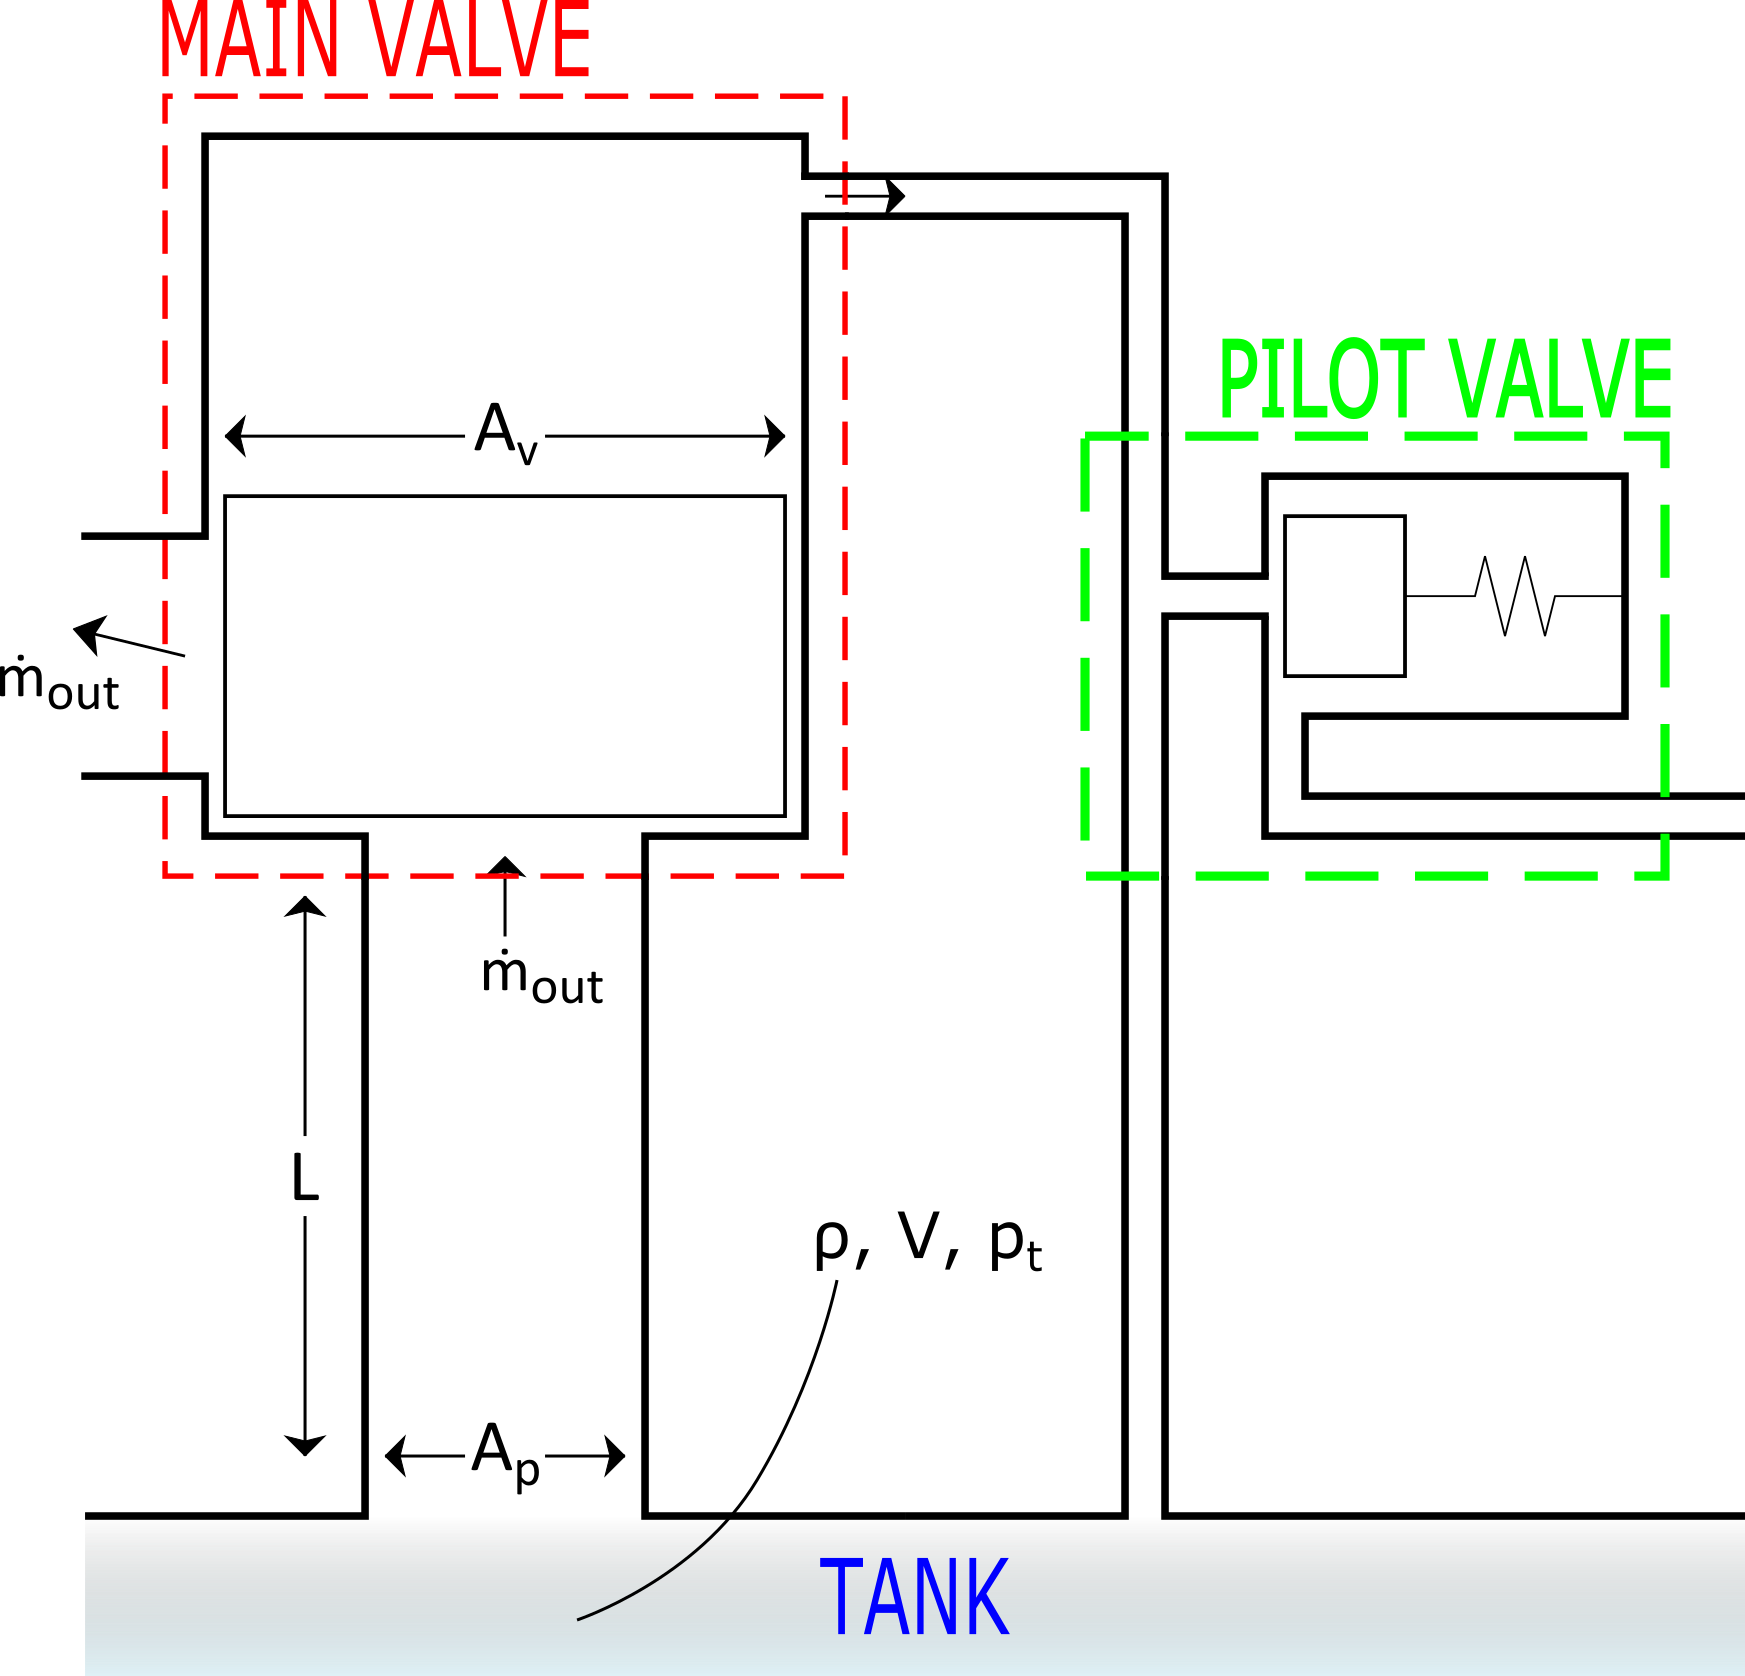
\includegraphics[width=\textwidth]{Diagrams/Diagram.png}
    \caption{Complete valve}
    \label{fig: DiagramComp}
    \end{subfigure}
    \hfill
    % Separate valve figures
    \begin{minipage}{0.3\textwidth}
        % MAIN DIAGRAM
        \begin{subfigure}{\textwidth}
        \centering
        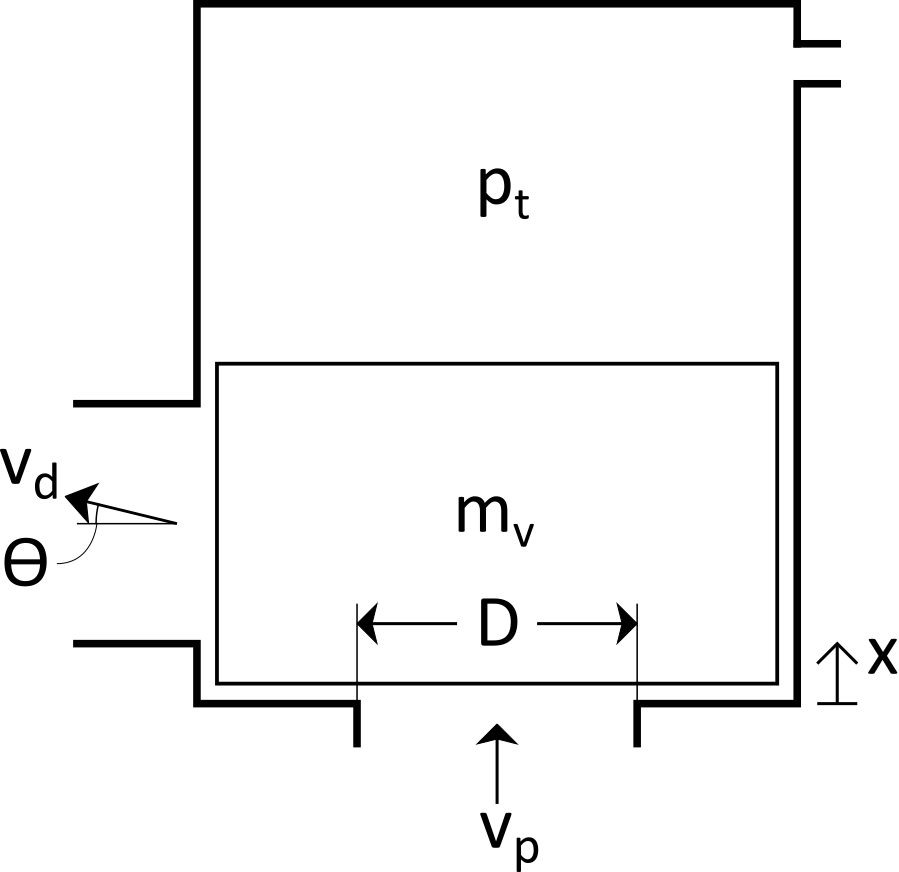
\includegraphics[width=\textwidth]{Diagrams/Diagram-Main.png}
        \caption{Main Valve}
        \label{fig: DiagramMain}
        \end{subfigure}
        % PILOT DIAGRAM
        \begin{subfigure}{\textwidth}
        \centering
        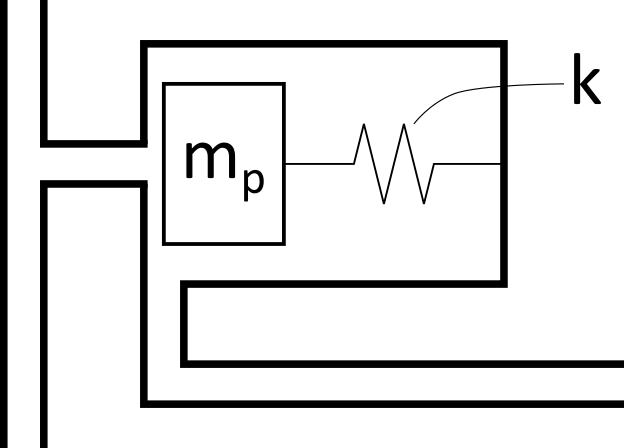
\includegraphics[width=\textwidth]{Diagrams/Diagram-Pilot.png}
        \caption{Pilot Valve}
        \label{fig: DiagramPilot}
        \end{subfigure}
    \end{minipage}
    % Figure caption and label
    \caption{Diagram of pilot-operated pressure relief valve}
    \label{fig: Diagram}
\end{figure}
%\end{sidewaysfigure}

% the end
\end{document}